% Generated fragments require trusted human review before compilation.
% This binder never requests shell escape or runs external tools.
\documentclass[11pt]{article}
% Trusted shared apparatus. Requires LuaLaTeX; never use shell escape.
\usepackage{fontspec}
\defaultfontfeatures{Ligatures=TeX}
\IfFontExistsTF{Noto Serif}{\setmainfont{Noto Serif}}{%
  \IfFontExistsTF{DejaVu Serif}{\setmainfont{DejaVu Serif}}{%
    \IfFontExistsTF{Times New Roman}{\setmainfont{Times New Roman}}{%
      \PackageError{gelfand-binder}{No configured Cyrillic serif font installed}{Install Noto Serif or DejaVu Serif, or select an installed Cyrillic font.}%
    }%
  }%
}
\IfFontExistsTF{Noto Sans}{\setsansfont{Noto Sans}}{%
  \IfFontExistsTF{DejaVu Sans}{\setsansfont{DejaVu Sans}}{\setsansfont{Arial}}%
}
\IfFontExistsTF{Noto Sans Mono}{\setmonofont{Noto Sans Mono}}{%
  \IfFontExistsTF{DejaVu Sans Mono}{\setmonofont{DejaVu Sans Mono}}{\setmonofont{Courier New}}%
}
\usepackage[a4paper,margin=22mm]{geometry}
\usepackage{amsmath,amssymb,amsthm,mathtools}
\usepackage{xcolor}
\usepackage{tikz}
\usepackage{tikz-cd}
\usetikzlibrary{arrows.meta,positioning,calc}
\usepackage{hyperref}
\hypersetup{unicode=true,colorlinks=true,linkcolor=blue,pdftitle={Gelfand transcription binder}}
\newtheorem{theorem}{Theorem}
\newtheorem{lemma}{Lemma}
\newtheorem{proposition}{Proposition}
\newtheorem{corollary}{Corollary}
\theoremstyle{definition}
\newtheorem{definition}{Definition}
\newtheorem{example}{Example}
\theoremstyle{remark}
\newtheorem{remark}{Remark}
\setlength{\parindent}{0pt}
\setlength{\parskip}{0.55em}
\setlength{\emergencystretch}{3em}
\newcommand{\SourcePage}[2]{%
  \clearpage\phantomsection\label{#1:source-page}%
  \addcontentsline{toc}{subsection}{#1}%
  {\small\sffamily\color{blue!60!black}Source scan frame: #1; visible page/leaf label: #2}\par\medskip%
}
\newcommand{\Unclear}[3]{%
  \begingroup\color{orange!70!black}%
  [Unresolved reading #1/#2: #3]\endgroup%
}
\newcommand{\Incomplete}[3]{%
  \par\begingroup\color{red!65!black}\textbf{Incomplete #1/#2:} #3\endgroup\par%
}
\newcommand{\SourceFigure}[3]{%
  \par\begingroup\color{blue!60!black}\textbf{\hyperref[#1:source-page]{Source figure #1/#2}:} #3%
  \par\textit{Consult the authoritative scan at this locator.}\endgroup\par%
}



% Reader layout only. Original diplomatic text is retained verbatim.
\setlength{\parskip}{0.35em}
\setlength{\emergencystretch}{4em}
\renewcommand{\SourcePage}[2]{%
  \par\addvspace{1em}\phantomsection\label{#1:source-page}%
  \addcontentsline{toc}{subsection}{#1}%
  {\footnotesize\sffamily\color{blue!55!black}#1%
    \def\givenlabel{#2}\def\nolabel{unlabelled}%
    \ifx\givenlabel\nolabel\else\quad[номер в источнике: #2]\fi
  }\par\nobreak\smallskip%
}
\renewcommand{\Unclear}[3]{%
  \begingroup\color{orange!65!black}%
  \ifmmode\text{[неясно: #3]}\else[неясно: #3]\fi\endgroup%
}
\renewcommand{\Incomplete}[3]{%
  \par\begingroup\color{red!60!black}\textbf{Неразобранный фрагмент:} #3%
  \endgroup\par%
}
\renewcommand{\SourceFigure}[3]{%
  \par\begingroup\color{blue!55!black}\textbf{Рисунок:} #3%
  \par{\small\textit{Исходный рисунок: \hyperref[#1:source-page]{#1}, #2.}}%
  \endgroup\par%
}
\hypersetup{pdftitle={Семинар И. М. Гельфанда. Дипломатическая транскрипция},pdfauthor={},pdfsubject={Русское рабочее издание с отмеченными сомнительными чтениями}}

\usepackage[normalem]{ulem}
\usepackage{newunicodechar}
\usepackage{adjustbox}
\newfontfamily\SourceSymbolFont{Segoe UI Symbol}
\newfontfamily\SourceCJKFont{MS Gothic}
\let\DiplomaticMathUnderline\underline
\renewcommand{\underline}[1]{\ifmmode\DiplomaticMathUnderline{#1}\else\uline{#1}\fi}
\newunicodechar{→}{\ifmmode\text{{\SourceSymbolFont\char"2192}}\else{\SourceSymbolFont\char"2192}\fi}
\newunicodechar{⇒}{\ifmmode\text{{\SourceSymbolFont\char"21D2}}\else{\SourceSymbolFont\char"21D2}\fi}
\newunicodechar{∀}{\ifmmode\text{{\SourceSymbolFont\char"2200}}\else{\SourceSymbolFont\char"2200}\fi}
\newunicodechar{∂}{\ifmmode\text{{\SourceSymbolFont\char"2202}}\else{\SourceSymbolFont\char"2202}\fi}
\newunicodechar{∈}{\ifmmode\text{{\SourceSymbolFont\char"2208}}\else{\SourceSymbolFont\char"2208}\fi}
\newunicodechar{∌}{\ifmmode\text{{\SourceSymbolFont\char"220C}}\else{\SourceSymbolFont\char"220C}\fi}
\newunicodechar{√}{\ifmmode\text{{\SourceSymbolFont\char"221A}}\else{\SourceSymbolFont\char"221A}\fi}
\newunicodechar{∞}{\ifmmode\text{{\SourceSymbolFont\char"221E}}\else{\SourceSymbolFont\char"221E}\fi}
\newunicodechar{∧}{\ifmmode\text{{\SourceSymbolFont\char"2227}}\else{\SourceSymbolFont\char"2227}\fi}
\newunicodechar{∩}{\ifmmode\text{{\SourceSymbolFont\char"2229}}\else{\SourceSymbolFont\char"2229}\fi}
\newunicodechar{∪}{\ifmmode\text{{\SourceSymbolFont\char"222A}}\else{\SourceSymbolFont\char"222A}\fi}
\newunicodechar{∫}{\ifmmode\text{{\SourceSymbolFont\char"222B}}\else{\SourceSymbolFont\char"222B}\fi}
\newunicodechar{∴}{\ifmmode\text{{\SourceSymbolFont\char"2234}}\else{\SourceSymbolFont\char"2234}\fi}
\newunicodechar{∼}{\ifmmode\text{{\SourceSymbolFont\char"223C}}\else{\SourceSymbolFont\char"223C}\fi}
\newunicodechar{≈}{\ifmmode\text{{\SourceSymbolFont\char"2248}}\else{\SourceSymbolFont\char"2248}\fi}
\newunicodechar{≠}{\ifmmode\text{{\SourceSymbolFont\char"2260}}\else{\SourceSymbolFont\char"2260}\fi}
\newunicodechar{≤}{\ifmmode\text{{\SourceSymbolFont\char"2264}}\else{\SourceSymbolFont\char"2264}\fi}
\newunicodechar{≥}{\ifmmode\text{{\SourceSymbolFont\char"2265}}\else{\SourceSymbolFont\char"2265}\fi}
\newunicodechar{⊕}{\ifmmode\text{{\SourceSymbolFont\char"2295}}\else{\SourceSymbolFont\char"2295}\fi}
\newunicodechar{⊗}{\ifmmode\text{{\SourceSymbolFont\char"2297}}\else{\SourceSymbolFont\char"2297}\fi}
\newunicodechar{①}{\ifmmode\text{{\SourceSymbolFont\char"2460}}\else{\SourceSymbolFont\char"2460}\fi}
\newunicodechar{②}{\ifmmode\text{{\SourceSymbolFont\char"2461}}\else{\SourceSymbolFont\char"2461}\fi}
\newunicodechar{③}{\ifmmode\text{{\SourceSymbolFont\char"2462}}\else{\SourceSymbolFont\char"2462}\fi}
\newunicodechar{④}{\ifmmode\text{{\SourceSymbolFont\char"2463}}\else{\SourceSymbolFont\char"2463}\fi}
\newunicodechar{Ⓗ}{\ifmmode\text{{\SourceSymbolFont\char"24BD}}\else{\SourceSymbolFont\char"24BD}\fi}
\newunicodechar{〃}{\ifmmode\text{{\SourceCJKFont\char"3003}}\else{\SourceCJKFont\char"3003}\fi}


% Reader revision 3. Annotation wording and candidates remain unchanged.
\setmainfont{NotoSerif-Regular.ttf}[Path=C:/Windows/Fonts/,ItalicFont=NotoSerif-Italic.ttf,BoldFont=NotoSerif-Bold.ttf,BoldItalicFont=NotoSerif-BoldItalic.ttf]
\usetikzlibrary{shapes.geometric,decorations.pathreplacing,decorations.markings,patterns,fit}
\newsavebox{\ReaderAnnotationBox}
\newcommand{\ReaderAnnotation}[1]{%
  \sbox{\ReaderAnnotationBox}{[неясно: #1]}%
  \ifdim\wd\ReaderAnnotationBox>.70\linewidth
    \parbox[t]{.70\linewidth}{\raggedright[неясно: #1]}%
  \else\usebox{\ReaderAnnotationBox}\fi%
}
\ExplSyntaxOn
\cs_new_protected:Npn \reader_unclear_candidate:n #1
 {
  \tl_set:Nx \l_tmpa_tl { \tl_to_str:n {#1} }
  % Text explicitly guarded inside a mathematical candidate remains math-safe.
  \regex_replace_all:nnN { \\(?:text|textrm|textnormal|textbf|operatorname)\s*\{[^{}]*\} } { } \l_tmpa_tl
  \regex_match:nVTF { [\x{0400}-\x{052F}] | \$ } \l_tmpa_tl
   { \ifmmode \text{\ReaderAnnotation{#1}} \else \ReaderAnnotation{#1} \fi }
   {
    \ifmmode
      [\text{неясно:~}#1]
    \else
      \regex_match:nVTF { [_^] | \\ } \l_tmpa_tl
       { \ensuremath{[\text{неясно:~}#1]} }
       { \ReaderAnnotation{#1} }
    \fi
   }
 }
\RenewDocumentCommand \Unclear { m m m }
 { \begingroup\color{orange!65!black}\reader_unclear_candidate:n{#3}\endgroup }
\ExplSyntaxOff
\newsavebox{\ReaderIncompleteBox}
\newcommand{\ReaderIncompleteNote}[1]{%
 \sbox{\ReaderIncompleteBox}{\textbf{Неразобранный фрагмент:} #1}%
 \ifdim\wd\ReaderIncompleteBox>.70\linewidth
  \parbox[t]{.70\linewidth}{\raggedright\textbf{Неразобранный фрагмент:} #1}%
 \else\usebox{\ReaderIncompleteBox}\fi%
}
\renewcommand{\Incomplete}[3]{%
 \ifmmode\text{\color{red!60!black}\ReaderIncompleteNote{#3}}%
 \else\leavevmode\begingroup\color{red!60!black}\ReaderIncompleteNote{#3}\endgroup\fi%
}
% Ragged right avoids stretching long untranslated abbreviations into margins.
\AtBeginDocument{\raggedright}
\newunicodechar{А}{\ifmmode\text{\char"410\relax}\else\char"410\relax\fi}
\newunicodechar{Б}{\ifmmode\text{\char"411\relax}\else\char"411\relax\fi}
\newunicodechar{В}{\ifmmode\text{\char"412\relax}\else\char"412\relax\fi}
\newunicodechar{Г}{\ifmmode\text{\char"413\relax}\else\char"413\relax\fi}
\newunicodechar{Д}{\ifmmode\text{\char"414\relax}\else\char"414\relax\fi}
\newunicodechar{Е}{\ifmmode\text{\char"415\relax}\else\char"415\relax\fi}
\newunicodechar{Ж}{\ifmmode\text{\char"416\relax}\else\char"416\relax\fi}
\newunicodechar{З}{\ifmmode\text{\char"417\relax}\else\char"417\relax\fi}
\newunicodechar{И}{\ifmmode\text{\char"418\relax}\else\char"418\relax\fi}
\newunicodechar{Й}{\ifmmode\text{\char"419\relax}\else\char"419\relax\fi}
\newunicodechar{К}{\ifmmode\text{\char"41A\relax}\else\char"41A\relax\fi}
\newunicodechar{Л}{\ifmmode\text{\char"41B\relax}\else\char"41B\relax\fi}
\newunicodechar{М}{\ifmmode\text{\char"41C\relax}\else\char"41C\relax\fi}
\newunicodechar{Н}{\ifmmode\text{\char"41D\relax}\else\char"41D\relax\fi}
\newunicodechar{О}{\ifmmode\text{\char"41E\relax}\else\char"41E\relax\fi}
\newunicodechar{П}{\ifmmode\text{\char"41F\relax}\else\char"41F\relax\fi}
\newunicodechar{Р}{\ifmmode\text{\char"420\relax}\else\char"420\relax\fi}
\newunicodechar{С}{\ifmmode\text{\char"421\relax}\else\char"421\relax\fi}
\newunicodechar{Т}{\ifmmode\text{\char"422\relax}\else\char"422\relax\fi}
\newunicodechar{У}{\ifmmode\text{\char"423\relax}\else\char"423\relax\fi}
\newunicodechar{Ф}{\ifmmode\text{\char"424\relax}\else\char"424\relax\fi}
\newunicodechar{Х}{\ifmmode\text{\char"425\relax}\else\char"425\relax\fi}
\newunicodechar{Ц}{\ifmmode\text{\char"426\relax}\else\char"426\relax\fi}
\newunicodechar{Ч}{\ifmmode\text{\char"427\relax}\else\char"427\relax\fi}
\newunicodechar{Ш}{\ifmmode\text{\char"428\relax}\else\char"428\relax\fi}
\newunicodechar{Щ}{\ifmmode\text{\char"429\relax}\else\char"429\relax\fi}
\newunicodechar{Ъ}{\ifmmode\text{\char"42A\relax}\else\char"42A\relax\fi}
\newunicodechar{Ы}{\ifmmode\text{\char"42B\relax}\else\char"42B\relax\fi}
\newunicodechar{Ь}{\ifmmode\text{\char"42C\relax}\else\char"42C\relax\fi}
\newunicodechar{Э}{\ifmmode\text{\char"42D\relax}\else\char"42D\relax\fi}
\newunicodechar{Ю}{\ifmmode\text{\char"42E\relax}\else\char"42E\relax\fi}
\newunicodechar{Я}{\ifmmode\text{\char"42F\relax}\else\char"42F\relax\fi}
\newunicodechar{а}{\ifmmode\text{\char"430\relax}\else\char"430\relax\fi}
\newunicodechar{б}{\ifmmode\text{\char"431\relax}\else\char"431\relax\fi}
\newunicodechar{в}{\ifmmode\text{\char"432\relax}\else\char"432\relax\fi}
\newunicodechar{г}{\ifmmode\text{\char"433\relax}\else\char"433\relax\fi}
\newunicodechar{д}{\ifmmode\text{\char"434\relax}\else\char"434\relax\fi}
\newunicodechar{е}{\ifmmode\text{\char"435\relax}\else\char"435\relax\fi}
\newunicodechar{ж}{\ifmmode\text{\char"436\relax}\else\char"436\relax\fi}
\newunicodechar{з}{\ifmmode\text{\char"437\relax}\else\char"437\relax\fi}
\newunicodechar{и}{\ifmmode\text{\char"438\relax}\else\char"438\relax\fi}
\newunicodechar{й}{\ifmmode\text{\char"439\relax}\else\char"439\relax\fi}
\newunicodechar{к}{\ifmmode\text{\char"43A\relax}\else\char"43A\relax\fi}
\newunicodechar{л}{\ifmmode\text{\char"43B\relax}\else\char"43B\relax\fi}
\newunicodechar{м}{\ifmmode\text{\char"43C\relax}\else\char"43C\relax\fi}
\newunicodechar{н}{\ifmmode\text{\char"43D\relax}\else\char"43D\relax\fi}
\newunicodechar{о}{\ifmmode\text{\char"43E\relax}\else\char"43E\relax\fi}
\newunicodechar{п}{\ifmmode\text{\char"43F\relax}\else\char"43F\relax\fi}
\newunicodechar{р}{\ifmmode\text{\char"440\relax}\else\char"440\relax\fi}
\newunicodechar{с}{\ifmmode\text{\char"441\relax}\else\char"441\relax\fi}
\newunicodechar{т}{\ifmmode\text{\char"442\relax}\else\char"442\relax\fi}
\newunicodechar{у}{\ifmmode\text{\char"443\relax}\else\char"443\relax\fi}
\newunicodechar{ф}{\ifmmode\text{\char"444\relax}\else\char"444\relax\fi}
\newunicodechar{х}{\ifmmode\text{\char"445\relax}\else\char"445\relax\fi}
\newunicodechar{ц}{\ifmmode\text{\char"446\relax}\else\char"446\relax\fi}
\newunicodechar{ч}{\ifmmode\text{\char"447\relax}\else\char"447\relax\fi}
\newunicodechar{ш}{\ifmmode\text{\char"448\relax}\else\char"448\relax\fi}
\newunicodechar{щ}{\ifmmode\text{\char"449\relax}\else\char"449\relax\fi}
\newunicodechar{ъ}{\ifmmode\text{\char"44A\relax}\else\char"44A\relax\fi}
\newunicodechar{ы}{\ifmmode\text{\char"44B\relax}\else\char"44B\relax\fi}
\newunicodechar{ь}{\ifmmode\text{\char"44C\relax}\else\char"44C\relax\fi}
\newunicodechar{э}{\ifmmode\text{\char"44D\relax}\else\char"44D\relax\fi}
\newunicodechar{ю}{\ifmmode\text{\char"44E\relax}\else\char"44E\relax\fi}
\newunicodechar{я}{\ifmmode\text{\char"44F\relax}\else\char"44F\relax\fi}
\newunicodechar{Ё}{\ifmmode\text{\char"401\relax}\else\char"401\relax\fi}
\newunicodechar{ё}{\ifmmode\text{\char"451\relax}\else\char"451\relax\fi}

\newunicodechar{æ}{\ifmmode\text{\char"E6\relax}\else\char"E6\relax\fi}
\newunicodechar{−}{\ifmmode\mathbin{\text{\SourceSymbolFont\char"2212\relax}}\else{\SourceSymbolFont\char"2212\relax}\fi}

\begin{document}
\begin{center}
{\Large Семинар И. М. Гельфанда}\par\medskip
{\LARGE Дипломатическая транскрипция}\par\bigskip
{\large Рабочее русское издание}\par\medskip
{\large Том 20 из 34. Архивная глава 020}\par\bigskip
Кадры GELFAND-P000981 -- GELFAND-P001000\par

\end{center}
\medskip
Сокращения, отменённые записи и сомнительные чтения сохранены.
Неразобранные фрагменты отмечены в тексте. Математические утверждения
источника переданы без молчаливых исправлений.

Это рабочее издание: сверка с рукописью продолжается. В текущем комплекте
учтены 1503 из 1527 кадров; 24 кадра пока представлены явными указателями
отсутствующего возврата. Полный журнал чтений и происхождения данных
сохранён в основном рабочем переплёте.

Границы кадров показаны небольшими синими указателями; печатный текст
продолжается без обязательного разрыва страницы после каждого кадра.
\bigskip\hrule\bigskip
\SourcePage{GELFAND-P000981}{unlabelled}
\underline{14/IX-81.}\qquad \underline{Сем. Гельфанда.}

\underline{И.М.Г.}\quad \underline{О контрагредиентных алгебрах Ли}

\underline{21/IX-81 г.}\qquad \underline{Сем. Гельфанда.}

\underline{С. Гельфанд.}

Читать по алгебрам Ли:

1. \underline{Диксмье} или \underline{Серр}, ч. 3 (1 и 2 не читать ни в коем случае)

[Под фамилией Диксмье, соединено короткой вертикальной чертой:]
Оберт. алгебры, гл. 1 --- учебная лит-ра.

2. \underline{Humphrey}, Lect. Notes, 831

модули со старш. весом для полупростых алгебр Ли.

(модули Верма́)

3. [Зачёркнуто: \Unclear{GELFAND-P000981}{biblio-cancel}{Mc Donald}]
\underline{Macdonald}\qquad Sem. \Unclear{GELFAND-P000981}{biblio-bourbaki}{Bourbaky}, июнь 1981 г.

4. Раб. \underline{Каца} и \underline{Габера}

5. \underline{И.М. Гельфанд и др.}\qquad Функц. ан., 5:1; 10:2

(Бернштейн, [зачёркнуто: \Unclear{GELFAND-P000981}{biblio-initial}{И}], И.М.Г., С.И.Г.)

6. \underline{Jantzen}, Lect. Notes, 750

7. \underline{Кац}, \underline{Каждан}\qquad Advances Math., 1979, \underline{34}, $N=1$.

\underline{И.М.Г.}\qquad $h$ --- вект. пр-во с базисом $h_1,\ldots,h_n$

$g$ --- полупростая алг. Ли
\begin{equation*}
\begin{aligned}
\operatorname{ad}x\colon g&\longrightarrow g\\
y&\longmapsto[x,y]
\end{aligned}
\end{equation*}
Скал. произв. Картана:
\Unclear{GELFAND-P000981}{trace-sign}{$(x,y)=\operatorname{tr}(\operatorname{ad}x-\operatorname{ad}y)$}
(\underline{Проверять} на алгебре матриц)

[Приписано под строкой:] и ортог. алг. 3-го пор.

\underline{И.М.Г.}\quad близко к станд. предст. гр. Лоренца лежат $\infty$-мерные предст.

Идея: в физику, ведь \Unclear{GELFAND-P000981}{lorentz-word}{смещение} гр. Лоренца приблизительно
(в наших масштабах это пренебрежительно)

\Unclear{GELFAND-P000981}{discussion-speaker}{Новиков}: малый сдвиг должен давать массу нейтрино

\underline{И.М.Г.}\qquad $h$ --- картановская подалгебра

\Unclear{GELFAND-P000981}{root-definition}{$g_\alpha$ наз. \underline{корнем}, если $[g_\alpha,h]=\alpha(h)g_\alpha$, $g_\alpha$}

($\alpha(\cdot)$ --- лин. ф-я на $h$, назыв. \underline{корнем})

\SourcePage{GELFAND-P000982}{12}
На $h$ появл. скал. произв. (двойное к картановскому).

Тогда получается \underline{$(\alpha,\alpha)>0$.}

Сущ. такие корни $\alpha_1,\alpha_2,\ldots,\alpha_n$, если $\alpha$ --- другой корень, то
\begin{equation*}
\alpha=\sum n_i\alpha_i,\qquad n_i\in\mathbb{Z}.
\end{equation*}
При этом все $n_i$ одного знака!

Если все $n_i\geq0$, то корень полож.

--- \textquotedblright\ --- $n_i\leq0$ --- \textquotedblright\ --- отриц.

Обязательно [зачёркнуто: \Unclear{GELFAND-P000982}{same-sign-cancel}{чтоб}] все $n_i$ одного знака!!

Их можно упорядочить

\underline{$\exists$ наиб. корень $\alpha_0$}

Кокорень:
\begin{equation*}
\underline{\alpha^{\vee}=\frac{2\alpha}{(\alpha,\alpha)}}
\end{equation*}
Набор \underline{кокорней} --- снова сист. корней (другая алгебра --- двойств. по Лэнглэндсу).

Строим отражение $w_\alpha\colon h\longrightarrow h$,
$w_\alpha(\lambda)=$ [зачёркнуто: \Unclear{GELFAND-P000982}{reflection-formula-cancel}{неразборчивый знак}]
$\lambda-(\alpha^{\vee},\lambda)\alpha$

$h$ и $h^*$ [зачёркнуто: \Unclear{GELFAND-P000982}{identify-cancel}{неразборчивое слово}]
отождествляем с пом. метрики

[Над следующей строкой зачёркнуто: \Unclear{GELFAND-P000982}{reflection-symbol-cancel}{$\alpha$}]

$w_\alpha$ --- отражение отн. плоскости, перпендик. $\alpha$.
\begin{equation*}
w_\alpha(\alpha)=-\alpha.
\end{equation*}
Группа, порожд. этими отр., конечна. \underline{Она наз. группой Вейля $W$.}

Для $sl(n)$ это [зачёркнуто: \Unclear{GELFAND-P000982}{symmetric-first-cancel}{гр}]
симметрич. [зачёркнуто: \Unclear{GELFAND-P000982}{symmetric-second-cancel}{перестановок}]
\Unclear{GELFAND-P000982}{group-order}{группа $n$-го порядка.}

$sl(3)\Rightarrow h$ --- 2-мерное пр-во

\Unclear{GELFAND-P000982}{sl-three-vectors}{$\sum\alpha_i=0$},
рисуем их все в пр-ве, но они лежат в плоск. $\sum_{i=1}^{3}x_i=0$

\begin{adjustbox}{max width=\linewidth}
\begin{tikzpicture}
\draw[->] (0,0) -- (1.4,0);
\draw[dashed] (1.4,0) -- (2.25,0);
\draw[->] (0,0) -- (-0.85,1.05);
\draw[dashed] (-0.85,1.05) -- (-1.1,1.42);
\draw[->] (0,0) -- (-0.85,-1.08);
\draw[dashed] (-0.85,-1.08) -- (-1.6,-2.02);
\end{tikzpicture}
\end{adjustbox}
\quad $\leftarrow$ получ. 3 вект. под углом $120^{\circ}$.

Свед. [зачёркнуто: \Unclear{GELFAND-P000982}{reflection-bottom-cancel}{неразборчивый знак}]
к отражениям: \underline{перестан. --- к транспозициям.}

отражен. соседних --- простые корни.

Все корни, получ. из простых преобраз. группы $W$.

$a_{ij}=(\alpha_i^{\vee},\alpha_j)$ --- матр. Картана.

\underline{Утв.}\quad $a_{ij}\in\mathbb{Z}$;
\Unclear{GELFAND-P000982}{matrix-props}{$a_{ij}\leq0$};
$a_{ij}=0\Rightarrow a_{ji}=0$

$(a_{ij})$ полож. определена.

Обратно: всякой такой матр. \Unclear{GELFAND-P000982}{matrix-converse}{соот.} алг. Ли.

Положим $\alpha_i^{\vee}=h_i$.

Тогда введём алг. Ли, опред. след. соотношениями:

\SourcePage{GELFAND-P000983}{unlabelled}
\Unclear{GELFAND-P000983}{serre-index-condition}{(*)}
\begin{equation*}
\left\{
\begin{aligned}
[e_i,f_j]&=\delta_{ij}h_i\\
[h_i,h_j]&=0\\
[h_i,e_j]&=a_{ij}e_j,\quad [h_i,f_j]=-a_{ij}f_j\\
(\operatorname{ad}e_i)^{1-a_{ij}}e_j&=0,\quad
(\operatorname{ad}f_i)^{1-a_{ij}}f_j=0
\end{aligned}
\right.
\end{equation*}

$V$ --- $g$-модуль

$\lambda\in h^*$ наз. весом, если это соб. знач., т.е. $\exists v\in V\setminus\{0\}$
\begin{equation*}
hv=\lambda(h)v.
\end{equation*}
$V_\lambda$ --- подпр-во соб. векторов с весом $\lambda$.

Пример $g$-модуля: $g$ с $\operatorname{ad}$.
\begin{equation*}
\dim V<\infty\quad\Rightarrow\quad V=\bigoplus V_\lambda
\end{equation*}
и все $\lambda$ лежат в решётке, порожд.
\Unclear{GELFAND-P000983}{weight-lattice}{корнями (кокорнями)}

\underline{Упорядочение $\lambda$:} лексикографически по коорд., порожд. простыми корнями.

$\exists!$ конечномерное предст., порожд. вектором старшего веса.

[Зачёркнуто: \Unclear{GELFAND-P000983}{vector-cancel}{$\forall$}]
$\alpha$ --- корень, $\lambda$ --- вес, $v_\lambda$ имеет вес $\lambda$ $\Rightarrow$

\Unclear{GELFAND-P000983}{vector-subscript}{$e_\alpha v_\alpha$ имеет вес $\alpha+\lambda$.}

\underline{Д-во.}
\begin{align*}
h(e_\alpha v_\alpha)
&=e_\alpha(hv_\alpha)+[h,e_\alpha]v_\alpha
=\lambda e_\alpha v_\alpha+\alpha e_\alpha v_\alpha=\\
&=(\lambda+\alpha)e_\alpha v_\alpha
\end{align*}

\underline{Теор. Картана}
[Зачёркнуто: \Unclear{GELFAND-P000983}{theorem-initial-cancel}{$\exists!$};
над строкой в обводке приписано: $\forall\lambda\geq0\exists!$]
конечномерн. предст.
[Зачёркнуто: \Unclear{GELFAND-P000983}{theorem-cancel}{для любого веса}]
\Incomplete{GELFAND-P000983}{theorem-cancel}{Точные слова короткой зачёркнутой фразы после «конечномерн. предст.» не восстановлены; приведённое чтение остаётся предположительным.}
такое, что

\Unclear{GELFAND-P000983}{theorem-vector}{$e_\alpha V_\lambda=0$},
$\forall\alpha\in\Delta_+$ (полож. корни)

(\underline{или} $\sim$ $\forall$ простого).

Введ. группу $e^\lambda$ след. образом:
\begin{equation*}
e^{(\lambda+\mu)}=e^\lambda e^\mu
\end{equation*}
$e$ --- буква.
\begin{equation*}
e^{\sum n_i\alpha_i}=(e^{\alpha_1})^{n_1}\cdots(e^{\alpha_n})^{n_n}
\end{equation*}

\underline{Характер представления:}
\begin{equation*}
\operatorname{ch}V\underset{\mathrm{def}}{=}\sum_\mu(\dim V_\mu)e^\mu
\end{equation*}

Введём [зачёркнуто: \Unclear{GELFAND-P000983}{rho-cancel}{кор}]
такой вес $\rho$:
\begin{equation*}
\rho(h_i)=1,\qquad i=1,\ldots,n
\end{equation*}
\begin{equation*}
h_i=\alpha_i^{\vee}
\end{equation*}
\underline{Ф-ла Вейля:}\qquad для предст. со старшим весом $\lambda$:

\SourcePage{GELFAND-P000984}{13}
[Зачёркнуто: \Unclear{GELFAND-P000984}{cancelled-character}{$\operatorname{ch}V(\lambda)=\dfrac{\det(w)e^{w(\lambda+\rho)}}{e^\rho\prod_{\alpha>0}(1-e^{-\alpha})}$}.]

\begin{equation*}
\operatorname{ch}V(\lambda)=
\frac{\displaystyle\sum_{w\in W}\det(w)e^{w(\lambda+\rho)}}
{e^\rho\displaystyle\prod_{\alpha>0}(1-e^{-\alpha})}.
\end{equation*}
$w(\lambda+\rho)$ — рез. действия $w$ на вес $\lambda+\rho$.
Отсюда, в частности,
\begin{equation*}
\sum\det(w)e^{w\rho}=e^\rho\prod_{\alpha>0}(1-e^{-\alpha}).
\end{equation*}
Для матриц это ф-ла
\begin{equation*}
\begin{vmatrix}
1&1&\cdots&1\\
x_1&x_2&\cdots&x_n\\
\vdots&\vdots&&\vdots\\
x_1^{n-1}&x_2^{n-1}&\cdots&x_n^{n-1}
\end{vmatrix}
=\prod(x_i-x_k).
\end{equation*}

\underline{Рудаков.}\qquad \underline{Алгебры Каца-Муди}

$A$ — $n\times n$-матр.
и набор образующих
\begin{equation*}
e_1,\ldots,e_n,\ f_1,\ldots,f_n,\ h_1,\ldots,h_n,
\end{equation*}
[Зачёркнутый знак:
\Unclear{GELFAND-P000984}{cancelled-generator}{неразборчиво}.]
\begin{equation*}
\varepsilon_1,\ldots,\varepsilon_n
\end{equation*}
и соотн.
\begin{equation*}
\begin{cases}
[h_i,h_j]=0\\
[h_i,e_j]=a_{ij}e_j\\
[h_i,f_j]=-a_{ij}f_j\\
[e_i,f_j]=\delta_{ij}h_i
\end{cases}
\end{equation*}
\begin{equation*}
\begin{cases}
[\varepsilon_i,\varepsilon_j]=0\\
[\varepsilon_i,e_j]=\delta_{ij}e_j\\
[\varepsilon_i,f_j]=-\delta_{ij}f_j\\
[\varepsilon_i,h_j]=0
\end{cases}
\end{equation*}
$F(A)$ — алгебра Ли, порожд. этими образ. и соотн.
\begin{equation*}
F(A)\supset\widetilde H=\langle h_i,\varepsilon_i\rangle.
\end{equation*}
$I$ — max идеал в $F(A)$, такой что образ $\{e_i,f_i,h_i,\varepsilon_i\}$
в $F(A)/I$ — линейно независ. система векторов.
Он существует и определен однозначно (max
«нетравмирующий»).
\begin{equation*}
\widetilde G(A)\overset{\mathrm{def}}=F(A)/I.
\end{equation*}

\SourcePage{GELFAND-P000985}{unlabelled}
$(2)$ — матр. 2-го пор. со следом $0$.
\begin{equation*}
\begin{pmatrix}2&-1\\-1&2\end{pmatrix}
\end{equation*}
[Зачёркнутый знак: \Unclear{GELFAND-P000985}{top-cancelled-mark}{неразборчиво}.]
Добавл. \underline{max нетравмирующая система}

\underline{Критерий конечномерности}

матр. \underline{симметризуема} (делается симметричной умн. на диагональную),
и \underline{положит. определена}, \underline{$2$ на главной диагонали}
\begin{equation*}
\widetilde G(A)\supset\underset{\substack{\vert\\\text{центр}}}{Z}
\end{equation*}
\begin{equation*}
Z\subset\langle h_i,\varepsilon_i\rangle
\end{equation*}
Надо ещё профакторизовать по max подпр-ву в $Z$, к-рое не пересек.
с лин. оболочкой $\{h_i\}$.
\begin{equation*}
J\subset Z
\end{equation*}
$(a_{ij})$ невырождена $\Rightarrow$ это уже не нужно

$(a_{ij})$ вырожд. $\Rightarrow$ корни лин. зависимые.
Мы добавл. [зачёркнуто: \Unclear{GELFAND-P000985}{cancelled-addition}{какие-то}
\Incomplete{GELFAND-P000985}{cancelled-addition-tail}{Оставшаяся зачёркнутая группа букв или знаков не прочитана.}],
\Unclear{GELFAND-P000985}{addition-clause}{что / чтоб} сделать их линейно независ.
Для этого формально расширяем $h$ с запасом
\begin{equation*}
J\subset Z,\qquad J\cap\langle h_i\rangle=0.
\end{equation*}
\begin{equation*}
G(A)\overset{\text{опр.}}=\widetilde G(A)/J_{\max}.
\end{equation*}
\begin{equation*}
H=\langle h_i,\varepsilon_i\rangle.
\end{equation*}
Опред. мн-во таких векторов $x\in G(A)$, что они собственные.
\begin{equation*}
G_\alpha=\{x\in G(A),\ \forall h\in H,\ [h,x]=\alpha(h)x\}.
\end{equation*}
\begin{equation*}
\alpha\in H^*
\end{equation*}
\underline{Корни}: те $\alpha$, для к-рых $G_\alpha$ ненулевые.

$A$ — матрица Картана, если

$1)$\quad $a_{ij}\in\mathbb Z$,\qquad $a_{ii}=2$,\qquad
\Unclear{GELFAND-P000985}{cartan-nonpositive}{$a_{ij}\le0$}

$2)$\quad $a_{ij}=0\ \Rightarrow\ a_{ji}=0$
[Зачёркнутый знак перед припиской:
\Unclear{GELFAND-P000985}{before-lemma-cancelled}{неразборчиво}.]
[Вписано над леммой: Пусть $A$ неприводимая
(\Unclear{GELFAND-P000985}{irreducible-parenthesis}{не расп. на ... клетки}).]
[Выше вписано: $u$ — вектор-столбец (в $R^n$), имеет смысл $Au\in R^n$.]

\underline{Лемма.}
$(\mathrm I)$ Если $Au\ge0$, то $u>0$ или $u=0$;
[зачёркнуто: \Unclear{GELFAND-P000985}{case-one-cancelled}{неразборчиво}]
$\det A\ne0$.

$(\mathrm{II})$\quad
\Unclear{GELFAND-P000985}{case-two-formula}{$Au\ge0\ \Rightarrow\ u=0$};
\quad $\exists u>0$, $Au=0$;\quad $\operatorname{rank} A=n-1$
\begin{equation*}
(\mathrm{III})\quad Au\ge0,\ u\ge0\ \Rightarrow\ u=0;
\quad \exists u>0:\ Au<0
\end{equation*}
Утверждение: верно одно и только одно из $(\mathrm I)$–$(\mathrm{III})$.

\SourcePage{GELFAND-P000986}{14}
$(\mathrm I)$ — конечномерные алг. Ли; они классифицируются

$(\mathrm{II})$ — расширенные.

$(\mathrm{III})$ — все остальные.

\underline{И. М. Г.} Тождества Рамануджана:
\begin{equation*}
\frac{1}{\displaystyle\prod_{n=1}^{\infty}(1-q^{5n-2})(1-q^{5n-3})}
=\sum_{m=0}^{\infty}\frac{q^{m(m+1)}}{(1-q)\cdots(1-q^m)}
\end{equation*}
\begin{equation*}
\frac{1}{\displaystyle\prod_{n=1}^{\infty}(1-q^{5n-1})(1-q^{5n-4})}
=\sum_{m=0}^{\infty}\frac{q^{m^2}}{(1-q)\cdots(1-q^m)}
\end{equation*}

$\underrightarrow{\text{С. Гельфанд.}}$

\underline{Модуль Верма.}

(см. Диксмье, Jantzen)

В $G(A)$ есть образующие $e_i,f_i,h_i$\qquad $H=\{h_i\}$

$\forall\lambda\in H^*$ построим модуль, порожд. одним вектором
\Unclear{GELFAND-P000986}{generator-vector-symbol}{$v$ / $v^{-}$} с условием
\begin{equation*}
(*)\quad\left[
\begin{aligned}
e_i v_0&=0\\
h v_0&=\lambda(h)v_0
\end{aligned}
\right.
\end{equation*}
\begin{equation*}
N_+=\{e_i\},\qquad N_-=\{f_j\}
\end{equation*}
\begin{equation*}
N_+v_0=0
\end{equation*}
$f_{i_1}f_{i_2}\cdots f_{i_k}v_0$ — такие буквы выписываем.

Соотн. $(*)$ наклад. и ещё те, к-рые диктуются $f_j$.
Легко получается, что
\begin{equation*}
h f_{i_1}\cdots f_{i_k}v_0
=[\lambda(h)-\alpha_{i_1}(h)-\cdots-\alpha_{i_k}(h)]
f_{i_1}\cdots f_{i_k}v_0,
\end{equation*}
т. е. $f_{i_1}\cdots f_{i_k}v_0$ — тоже весовой вектор

Модуль, \Unclear{GELFAND-P000986}{module-abbrev}{соотв. / соб.} хар. $\lambda$, наз. $M(\lambda)$.
\begin{equation*}
\operatorname{Hom}(M(\lambda),M(\mu))=
\begin{cases}0\text{ или}\\\mathbb C\end{cases}
\end{equation*}
— и тогда любой нетрив. гомом. явл. вложением

\underline{Теорема.} Если $\operatorname{Hom}(M(\lambda),M(\mu))\ne0$, то
\begin{equation*}
1)\quad \lambda=\mu-\sum n_i\alpha_i
\quad\text{для нек-рых }n_i\ge0\text{ целых}
\end{equation*}
$2)$\quad\Unclear{GELFAND-P000986}{rho-shift}{$\lambda-\rho=w(\mu-\rho)$}
\quad для нек-рого $w\in W$

($\rho$ — \underline{полусумма} всех полож. корней — см. выше).
\begin{equation*}
3)\quad\lambda-\rho=s_{\delta_1}\cdots s_{\delta_k}(\mu-\rho)
\end{equation*}
($s_\delta$ — отраж. отн. любых корней, не обяз. простых)
и
\begin{equation*}
\begin{aligned}
&-s_{\delta_i}\cdots s_{\delta_k}(\mu-\rho)
+s_{\delta_{i-1}}s_{\delta_i}\cdots s_{\delta_k}(\mu-\rho)
=m_i\delta_{i-1},\\
&m_i\le0,\quad m_i\in\mathbb Z.
\end{aligned}
\end{equation*}
$1)$–$3)$ — уже достаточны для нетривиальности
\Unclear{GELFAND-P000986}{hom-sufficiency-final}{$\operatorname{Hom}(M(\lambda),M(\lambda))$}

\SourcePage{GELFAND-P000987}{unlabelled}
\underline{\Unclear{GELFAND-P000987}{task-title}{Задача}} (И.М.Г.) (не банальная)

$(a_{ij})$ — матр. Картана; уд. усл. 1) и 2)

Какова размерность пр-ва корней?

$\forall$ корня строятся \Unclear{GELFAND-P000987}{task-linear-abbrev}{ли.} незав. слова и т.д.

\bigskip
\underline{28.9.81 г.}\qquad\underline{Сем. Гельфанда}

\underline{\Unclear{GELFAND-P000987}{speaker-name}{Зайферт} (?)} (Париж)

\SourceFigure{GELFAND-P000987}{annotation-icon}{Справа от заголовка маленький жёлтый значок с чёрным контуром, нижним выступом и тремя чёрными горизонтальными штрихами внутри.}

$(X,G)$ — произв. гр. преобразований

$\mathcal P(X)$ — мн-во подмн-в $X$

$\mathcal F\subset\mathcal P(X)$ определяется след. образом:

[Над началом следующей строки зачёркнуто: \Unclear{GELFAND-P000987}{cancel-above-definition}{неразборчиво}.]

[Перед $S$ зачёркнуто: \Unclear{GELFAND-P000987}{cancel-before-definition}{неразборчиво}.]
\begin{equation*}
S\in\mathcal F\underset{\mathrm{def}}{\Longleftrightarrow}
\forall x\notin S,\ \exists g\in G,\ gs=s,\ \forall s\in S,\ gx\ne x
\end{equation*}

$G$ действует на $\mathcal F$
\begin{equation*}
1\longrightarrow G_S\longrightarrow
\underset{\substack{\Vert\\\{g\mid gS=S\}}}{G^S}
\overset{\substack{\text{\underline{ограничение}}\\\downarrow}}{\longrightarrow}
\overline{G^S}\longrightarrow1
\qquad\text{(расширение)}
\end{equation*}

Здесь
\begin{equation*}
G_S=\bigcap_sG_s,\qquad G_s=\operatorname{St}_G(s)
\end{equation*}

$\mathcal F$ облад. след. форм. св-вом:

замкнуто отн. любых пересечений
\begin{equation*}
S_i\in\mathcal F,\ \forall i\ \Rightarrow\ \bigcap_{i\in I}S_i\in\mathcal F
\end{equation*}

$(I,<)$ — частично упоряд. мн-во. Рассм. ф-и $f:I\to\mathcal F$, облад. св-вом:
\begin{equation*}
\{f:I\to\mathcal F\mid f(i)\subseteq f(j)\Longleftrightarrow i\le j\}
\end{equation*}

Тогда $G$ действует на этом мн-ве.

Фиксируя $(I,<)$, можно, в частности, рассмотреть все такие ф-и
\begin{equation*}
(\overline{\mathcal F}_I,G)=\{f:I\to\mathcal F:\ \text{как выше и при том}
\end{equation*}
[Над строкой вписано: \Unclear{GELFAND-P000987}{flag-if-insertion}{если}; под вставкой большой V-образный знак.]
$i<i'$ [зачёркнуто: \Unclear{GELFAND-P000987}{flag-cancel}{неразборчиво}]
минимальная цепь (2 соседних элем.) в $(I,<)$
$\Rightarrow f(i)$ \Unclear{GELFAND-P000987}{flag-strict-inclusion}{$\underset{\ne}{\subset}$}
$f(i')$ — тоже мин. цепь $\}$

Тогда $G$ тоже действ. на мн-ве таких ф-ий.

Из форм. св-ва устойч. отн. пересеч.
\begin{equation*}
S\subseteq X\rightsquigarrow
\underset{\text{(замык.)}}{S^{cl}}
=\bigcap_{\substack{T\in\mathcal F\\T\supseteq S}}T
\end{equation*}
\Unclear{GELFAND-P000987}{closure-terminal-zero}{$=(0)$}

\SourcePage{GELFAND-P000988}{15}
\begin{equation*}
x\in X\Rightarrow\text{опред. }\{x\}^{cl}\underset{\mathrm{def}}{=}
\text{прямая, прох. через эту точку}
\end{equation*}

$G$ [вписано: действ.] транзитивно
$\Rightarrow\{x\}^{cl}$ — мн-во точек \Unclear{GELFAND-P000988}{stabilizer-equality}{с тем же стабилизатором}, что и $x$

$G_x$ — обозначение стабилизатора.

Идея: однократная транзитивность $\Rightarrow$ многократную транзитивность
\begin{equation*}
\exists x:\ \{x\}^{cl}\underset{\ne}{\supset}x
\Rightarrow\text{группа не может действ. дважды транзитивно}
\end{equation*}

\begin{center}
\begin{adjustbox}{max width=\linewidth}
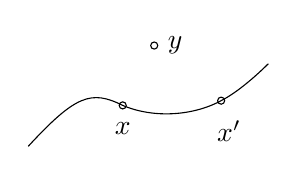
\begin{tikzpicture}[x=1cm,y=1cm]
\draw (0,0) .. controls (0.6,0.65) and (0.8,0.72) .. (1.2,0.52)
.. controls (1.6,0.35) and (2.1,0.39) .. (2.45,0.58)
.. controls (2.65,0.68) and (2.9,0.90) .. (3.05,1.05);
\draw (1.2,0.52) circle (0.045);
\draw (2.45,0.58) circle (0.045);
\draw (1.6,1.28) circle (0.045);
\node[below] at (1.2,0.43) {$x$};
\node[below] at (2.55,0.45) {$x'$};
\node[right] at (1.65,1.28) {$y$};
\end{tikzpicture}
\end{adjustbox}
\end{center}

$(x,y)\mapsto(x,x')$ невозможно, т.к. $\{x\}^{cl}$
\Unclear{GELFAND-P000988}{impossible-tail}{неразборчиво}

На $\overline{\mathcal F}_I$ уже может действовать дважды транзитивно

\underline{Пример}

дважды транзит. на $F\Longleftrightarrow$ транзит. на $(F\times F)\setminus\Delta$
\begin{equation*}
\forall x\in F,\ G_x\text{ должно транзит. действ. на }F\setminus\{x\}
\end{equation*}

\begin{center}
\begin{adjustbox}{max width=\linewidth}
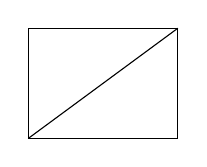
\begin{tikzpicture}[x=1cm,y=1cm]
\draw (0,0) -- (0,1.4) -- (1.9,1.4) -- (1.9,0) -- (0,0);
\draw (0,0) -- (1.9,1.4);
\end{tikzpicture}
\end{adjustbox}
\end{center}

Конец будет такой: для

$B,N,T,W,P$

даётся аксиоматич. обобщение, при к-ром имеет смысл разлож. Брюа.

\underline{При нек-рых усл. на действие:}

(i)
\begin{equation*}
\overline{\mathcal F}_{\max}=\{\max\ \text{вполне упоряд. цепь}\quad
S_1<S_2<\cdots<S_i<\cdots
\end{equation*}
[Зачёркнуто: \Unclear{GELFAND-P000988}{axiom1-cancel-end}{неразборчиво}.]
$S_i\in$ [зачёркнуто: \Unclear{GELFAND-P000988}{axiom1-cancel-family}{неразборчиво}] $\mathcal F\}$

[Под $\overline{\mathcal F}_{\max}$:] (Флаги)

\underline{транзит. относит. $G$}

(ii)
\begin{equation*}
\forall S:\ \dim(S)=\text{длина }\max\text{ флага},\ <+\infty
\end{equation*}
[Под $S$ приписано $\mathcal F$ со стрелкой вверх.]

[Под $\dim(S)$ зачёркнуто: \Unclear{GELFAND-P000988}{axiom2-cancel-under-dim}{неразборчиво}.]

[Под словами «длина $\max$ флага»: зачёркнуто \Unclear{GELFAND-P000988}{axiom2-cancel-before-ending}{неразборчиво}, затем:] заканчив. $S$.

(iii)
\begin{equation*}
S,S'\subseteq T,\quad\dim S+\dim S'>\dim(T)
\Rightarrow S\cap S'\ne\bigcap_{\mathcal F\ni T'}T'
\end{equation*}

(iv) $\forall S\in\mathcal F$, если $\{x\}^{cl}\cap S=$
\Unclear{GELFAND-P000988}{axiom4-zero}{$(\varnothing)^{cl}$}, то
\begin{equation*}
G^S\cap G^{\{x\}^{cl}}
\underset{\text{отобр. \underline{\underline{на}}}}{\longrightarrow}
\overline{G^S}
\end{equation*}

Тогда
\begin{equation*}
G=\coprod_WG^f wG^f\qquad\text{(несвязное объед.)}
\end{equation*}
(двойной смежн. класс)

где
\begin{equation*}
G^f=\bigcap_IG^{f(i)},\qquad f:I\to\mathcal F
\end{equation*}
[Под $G^f$, с выносной чертой:] стабилизатор $\max$ флага.
\begin{equation*}
W=N/T
\end{equation*}

[Над $f$ приписано: здесь.]
\begin{equation*}
\{f:I\to\mathcal F,\quad S_1<S_2<S_3<S_4<\cdots
\end{equation*}
\Unclear{GELFAND-P000988}{bottom-left-arrow}{$\leftarrow$}
любая $\max$ цепь $\}$

\SourcePage{GELFAND-P000989}{unlabelled}
\underline{Задачи.} (И.М.Г.)

Описать 2-стор. классы смежности
\begin{enumerate}
\item $U(n)\backslash GL(n)/U(n)$
\item $B(n)\backslash GL(n)/B(n)$

[К левому $B(n)$ снизу проведена наклонная черта с подписью «треуг.».]
\item $U(n)\backslash GL(n)/B(n)$
\end{enumerate}

$\forall\ \max$ флаг получ. так:
\begin{equation*}
f(i)=\mathrm{cl}(\{e_j\}_{j\leq i}),\quad
\text{где }\{e_j\}\text{ — точки в }X.
\end{equation*}
\begin{equation*}
C_i=\mathrm{cl}(\{e_i\})
\end{equation*}
\begin{equation*}
N=\{g\mid g\text{ переставляет }\{C_i\}\}
\end{equation*}
и мы имеем:

\SourceFigure{GELFAND-P000989}{middle-group-sequence}{Горизонтальная последовательность: первый знак переписан поверх другого; далее стрелки направо к $T$, $N$, $W$, $1$. Начальный знак похож на $1$, исправленную поверх $0$, либо на $0$, исправленный поверх $1$.}

$T$ сост. из тех, к-рые оставл. на месте каждое $C_i$;

$W=N/T$ по опред.

Докладчик не знает примеров, отл. от классических, где вып. все аксиомы.
Но: есть примеры, где разлож.
\Unclear{GELFAND-P000989}{lower-cancelled-word}{[Зачёркнуто короткое слово: «не»?]}
есть, хотя аксиомы не выполн.

\underline{Зелевинский.}

О работе \underline{S. Abeasis, A. Del Fra, H. Kraft.}

\underline{The geometry of repres. of $A_m$}, Math. Ann., 256, N.3,
\Unclear{GELFAND-P000989}{lower-bibliography-pages}{401–418 [или 402–418]}, (1981).

$A_m$ — колчан

\SourceFigure{GELFAND-P000989}{lower-quiver}{Слева $A:$; на одной горизонтали $V_1$, $V_2$, многоточие, $V_m$. Между $V_1$ и $V_2$ стрелка направо с надписью $A_1$; от $V_2$ к многоточию стрелка направо с надписью $A_2$; последняя стрелка к $V_m$ имеет надпись $A_m$. У её левого конца есть дополнительные штрихи: обратный наконечник либо повторная обводка; требуется сверка направления.}

— это представл. колчана серии $A_m$.

Здесь действ. группа

\Unclear{GELFAND-P000989}{bottom-group-index}{$GL(V_i)$ [или $GL(V_1)$]}$\times\cdots\times GL(V_m)$.

Орбиты — предст. с точн. до эквив.

Орбит конечное число. Они \Unclear{GELFAND-P000989}{bottom-description-abbrev}{допус. [или допуск.]} явное опис.

Их замык. — хорошие мн-ия (нормальные, Коэн —
\Unclear{GELFAND-P000989}{bottom-cohen-macaulay}{Маколеевы [или Маколевы / Маколея]}
и т.п.).

\SourcePage{GELFAND-P000990}{16}
\Unclear{GELFAND-P000990}{top-cancelled-word}{[Зачёркнуто: «Их»?]}
Они аналогичны клеткам Шуберта и многочлены описывают
предст. $p$-адич. групп, как геом. клеток Шуберта связана с предст.
классич. групп.

Для
\begin{adjustbox}{max width=\linewidth}
\begin{tikzcd}
V_1 \arrow[r,"A_1"] & V_2
\end{tikzcd}
\end{adjustbox}
возникают детерминантные мн-ия.

Описание орбит:

\SourceFigure{GELFAND-P000990}{upper-composition-arrow}{На одной горизонтали $V_i$ и $V_j$, между ними стрелка направо. Под стрелкой подпись «композ.». Под $V_i$ отдельный переписанный или зачёркнутый знак, похожий на $A$ либо $U$; его чтение и роль неясны.}

Надо задать \underline{ранги всевозм. композиций} $r_{ij}$.

Должна быть вып. система нер-в.

Есть другое опис. через кратности вхождений.

\underline{\underline{19/X-81г.}} \underline{Сем. Гельфанда.}

\underline{Кириллов.}

Как устр. алгебра Ли с образующими $x,y$ и соотн.
\begin{equation*}
(\operatorname{ad}x)^{a+1}y=0,\qquad
(\operatorname{ad}y)^{b+1}x=0,\qquad a,b\in\mathbb{N}.
\end{equation*}

\begin{center}
\begin{adjustbox}{max width=\linewidth}
\begin{tikzpicture}[x=0.8cm,y=0.65cm]
\draw[->] (0,0) -- (6,0) node[right] {$a$};
\draw[->] (0,0) -- (0,-6) node[below] {$b$};
\node at (0.5,0.4) {$1$};
\node at (1.3,0.4) {$2$};
\node at (2.1,0.4) {$3$};
\node at (3,0.4) {$4$};
\node at (-0.4,-0.5) {$1$};
\node at (-0.4,-1.3) {$2$};
\node at (-0.4,-2.1) {$3$};
\node at (-0.4,-2.9) {$4$};
\node at (0.5,-0.5) {$3$};
\node at (1.3,-0.5) {$4$};
\node at (2.1,-0.5) {$6$};
\node at (3,-0.5) {$\infty$};
\node at (0.5,-1.3) {$4$};
\node at (1.3,-1.3) {$\infty$};
\node at (2.1,-1.3) {$?$};
\node at (0.5,-2.1) {$6$};
\node at (1.3,-2.1) {$?$};
\node at (0.5,-2.9) {$\infty$};
\draw[->] (8,-1.1) -- (6.1,-1.1);
\node[anchor=west,align=left] at (8.2,-1.1) {размерности в тех случаях,\\когда они известны.};
\end{tikzpicture}
\end{adjustbox}
\end{center}

\underline{Без соотношений} число коммов бистепени $k,\ell$ равно:
\begin{equation*}
d(k,\ell)=\frac{1}{k+\ell}\sum_{d\mid(k,\ell)}
\mu(d)\,\frac{\left(\frac{k}{d}+\frac{\ell}{d}\right)!}
{\frac{k}{d}!\,\frac{\ell}{d}!}.
\end{equation*}

$k=n$, $\ell=n+1$ $\Rightarrow$ $n$-е число Каталана

($=$ число способов расстан. скобок в
неассоциат. произведении $x\cdot x\cdot\ldots\cdot x$.)

[Слева: $(\sim)$.]

Другой вопрос: оберт. алгебра.

\underline{Соотн:}
\begin{align*}
0&=x^{a+1}y-\binom{a+1}{1}x^ayx+\binom{a+1}{2}x^{a-1}yx^2+\ldots\,,\\
0&=y^{b+1}x-\binom{b+1}{1}y^bxy+\binom{b+1}{2}y^{b-1}xy^2-\ldots\,.
\end{align*}
\Unclear{GELFAND-P000990}{lower-relation-signs}{[В первой строке перед многоточием написан $+$, во второй $-$.]}

$V$ — вект. пр-во, \qquad $S(\bar V)=e^{\bar V}$ — симм. алгебра

[Под «$V$ — вект. пр-во»: «(градуир.)».]

\Unclear{GELFAND-P000990}{bottom-hilbert-letter}{$p(t)$ [или $\rho(t)$]}$=\sum t^k\dim V_k$ — многочлен Гильберта.


% GELFAND-0107. Diplomatic transcription from the ten supplied original PNG frames.
% Editorial descriptions are bracketed; unresolved evidence is linked to the JSON ledger.
% REVIEW coordinates: original pixels, origin at upper left; box=(left,top,right,bottom).
% REVIEW scale: nearest-neighbour raster enlargement; no additional source detail is implied.
% Direct visual inspection; no OCR. No external mathematical reconstruction.
\SourcePage{GELFAND-P000991}{unlabelled}
% REVIEW original: 2415x3480; full frame inspected.
% REVIEW top-lines: box=(190,45,2030,350); scale=2x.
% REVIEW series: box=(275,355,1900,700); scale=2x.
% REVIEW series-introduction: box=(245,290,820,505); scale=3x.
% REVIEW word-and-sums: box=(445,675,1390,1050); scale=3x.
% REVIEW lower-region: box=(130,1040,2300,1910); scale=2x.
% REVIEW diagram-margin: box=(135,1550,490,1830); scale=3x.
% REVIEW book-name: box=(535,1740,1860,1885); scale=3x.
% REVIEW second-cancellation: box=(665,510,920,670); scale=5x.
% REVIEW small-series-coefficient: box=(875,560,1120,680); scale=5x.
% REVIEW small-series-terms: box=(1100,540,1400,690); scale=5x.
% REVIEW divisor-sum: box=(1460,460,1820,675); scale=4x.
$k$ — вес $\Rightarrow$ возникает вес на $S(V)$
$\Rightarrow$ градуир. на $S(V)$
$\Rightarrow$ полином Гильберта вычисляется $P(t)$ для $S(V)$
(или форм. ряд).

Связь:

[Зачёркнуто: \Unclear{GELFAND-P000991}{series-cancelled-01}{неразборчиво}.]
\begin{equation*}
\ln P(t)=\sum \frac{C_k}{k}t^k;
\end{equation*}
[Зачёркнуто: \Unclear{GELFAND-P000991}{series-cancelled-02}{неразборчиво}.]
\begin{equation*}
p(t)=\sum \frac{c_k}{k}t^k,
\qquad C_k=\sum_{d\mid k}c_d.
\end{equation*}
\begin{equation*}
\underline{x^{k_1}y^{l_1}x^{k_2}y^{l_2}\ldots x^{k_n}y^{l_n}}
\end{equation*}
\begin{equation*}
k_1+k_2+\ldots+k_n=k,\qquad
l_1+l_2+\ldots+l_n=l.
\end{equation*}
Лексикограф. упоряд.

\underline{$y$ старше $x$}. \qquad $x<y$.

\underline{И.М.Г.} \quad \underline{комбин. задачи}

$m_1\le m_2\le m_3\le m_4$ — \underline{фиксир.}

\begin{center}
\begin{adjustbox}{max width=\linewidth}
\begin{tikzpicture}[x=1cm,y=1cm]
\node[draw,circle,inner sep=1.8pt] (a1) at (0,0) {};
\node[draw,circle,inner sep=1.8pt] (a2) at (1.2,0) {};
\node[draw,circle,inner sep=1.8pt] (a3) at (2.4,0) {};
\node[draw,circle,inner sep=1.8pt] (a4) at (3.6,0) {};
\node[draw,circle,inner sep=1.8pt] (b1) at (.6,-.8) {};
\node[draw,circle,inner sep=1.8pt] (b2) at (1.8,-.8) {};
\node[draw,circle,inner sep=1.8pt] (b3) at (3,-.8) {};
\node[draw,circle,inner sep=1.8pt] (c1) at (1.2,-1.6) {};
\node[draw,circle,inner sep=1.8pt] (c2) at (2.4,-1.6) {};
\node[draw,circle,inner sep=1.8pt] (d1) at (1.8,-2.4) {};
\draw (a1)--(b1)--(a2)--(b2)--(a3)--(b3)--(a4);
\draw (b1)--(c1)--(b2)--(c2)--(b3);
\draw (c1)--(d1)--(c2);
\node[align=center] (m) at (-1.1,-2) {между\\$m_1$ и $m_2$\\(вкл. концы)};
\draw[->] (m.north east)--(b1);
\end{tikzpicture}
\end{adjustbox}
\end{center}

\underline{ск. таблиц?}

(= сколько предст. $SL(4)$ с зад. старшим весом?)

см. добавл. к книге Гельфанд–Минлос–Шапиро.

\SourcePage{GELFAND-P000992}{unlabelled}
% REVIEW original: 2416x3480; full frame inspected.
% REVIEW heading-super-space: box=(280,1370,1900,1870); scale=2x.
% REVIEW coordinates-real-form: box=(330,1850,2290,2480); scale=2x.
% REVIEW surface-transformations: box=(290,2460,2300,3370); scale=2x.
% REVIEW grassmann-algebra: box=(310,1710,1570,1855); scale=3x.
% REVIEW points-or-rows: box=(800,1860,1230,1990); scale=4x.
% REVIEW functor-parenthesis: box=(1470,2150,2270,2285); scale=3x.
% REVIEW transformations-word: box=(830,2980,1320,3100); scale=4x.
% REVIEW crossed-algebra-phrase: box=(875,1720,1260,1845); scale=5x.
% REVIEW superscript-algebra: box=(685,1710,760,1785); scale=10x.
% REVIEW functor-words-second-look: box=(1570,2170,2175,2280); scale=5x.
% REVIEW transformation-line-second-look: box=(345,3005,1230,3125); scale=3x.
\underline{16.11.81г.} \qquad \underline{Сем. Гельфанда.}

\underline{А.С. Шварц.} \qquad \underline{Геометрия супергравитации.}

$\mathbb R^{p,q}$ — суперпр-во \qquad
$(x^1,\ldots,x^p,\theta^1,\ldots,\theta^q)$.

$\Lambda$ — грассм. алг.
[Над сокращением вписан знак:
\Unclear{GELFAND-P000992}{algebra-insertion}{г или 4}.]
[Зачёркнуто: \Unclear{GELFAND-P000992}{algebra-cancelled-01}{неразборчиво}.]
[Зачёркнуто:
\Unclear{GELFAND-P000992}{algebra-cancelled-02}{с градуировкой}.]
(над $\mathbb R$).

$\mathbb R^{p,q}_{\Lambda}$ — пр-во строчек
$(x^1,\ldots,x^p,\theta^1,\ldots,\theta^q)$,
где $x^j$ — чётные элем. $\Lambda$,
$\theta^j$ — нечётные элем. $\Lambda$.

Нужно рассм. это как функтор от $\Lambda$
(\Unclear{GELFAND-P000992}{functor-parenthesis}{неудобно}
фиксировать $\Lambda$).
Получается $\mathbb R^{p,q}$.

$\mathbb C^{p,q}$ опред. аналогично и в нём опред. инволюция.

\medskip
Рассм. $\mathbb C^{4,2}$ \qquad $(x^m,\theta^\alpha)=z^A$.
\begin{equation*}
\dim_{\mathbb C}\mathbb C^{4,2}=(4,2),\qquad
\dim_{\mathbb R}(\mathbb C^{4,2})=(8,4).
\end{equation*}
В нём рассм. веществ. подмн-зие $\Omega\subset\mathbb C^{4,2}$.
[Под $\Omega$ подписано: $(4,4)$; стрелка от «$\mathbb R$-dim».]

$\Omega$ выд. ур-ями
\begin{equation*}
f^k(z,\bar z)=0,
\end{equation*}
$f^k$ — чётные вещественные, \quad $k=1,2,3,4$.

Рассм. в $\mathbb C^{4,2}$ аналит. преобр-я:
\begin{equation*}
\begin{cases}
\widetilde{x}^{a}=\lambda^{a}(x,\theta),\\
\widetilde{\theta}^{\alpha}=\lambda^{\alpha}(x,\theta)
\end{cases}
\qquad
\text{(не завис. от $\bar x,\bar\theta$)}.
\end{equation*}

\SourcePage{GELFAND-P000993}{40}
% REVIEW original: 2416x3480; full frame inspected.
% REVIEW upper-group-ber: box=(155,40,2240,765); scale=2x.
% REVIEW functional-graph: box=(165,765,2290,1470); scale=2x.
% REVIEW supergravity-action: box=(175,1460,2240,2110); scale=2x.
% REVIEW levi-form: box=(170,2110,2260,3320); scale=2x.
% REVIEW group-parenthesis: box=(775,125,2175,260); scale=3x.
% REVIEW preserved-volume-word: box=(275,320,1360,435); scale=3x.
% REVIEW functional-cancellation: box=(1030,765,1455,905); scale=5x.
% REVIEW superfield-argument: box=(1180,1560,1600,1680); scale=5x.
% REVIEW correspondence-line: box=(235,1660,1920,1780); scale=3x.
% REVIEW levi-first-form: box=(185,2360,1690,2480); scale=3x.
% REVIEW levi-cancelled: box=(325,2815,475,2910); scale=6x.
% REVIEW variation-line: box=(280,2010,1250,2120); scale=3x.
% REVIEW variation-last-word: box=(1000,2020,1240,2115); scale=5x.
Они образуют супергруппу $L$.

(Группа зависит от $\Lambda$ и всё вместе — функтор из грассм. алг.
в обычные группы — супергруппы.)

Рассм. те, к-рые сохраняют \underline{суперобъём}.
\begin{equation*}
\widetilde z^{A}=\lambda^{A}(z).
\end{equation*}
Сохр. объёма:
\begin{equation*}
\operatorname{Ber}\frac{\partial\widetilde z^{A}}{\partial z^{B}}=1.
\end{equation*}
Будем рассм. ф-ал
\begin{equation*}
S(\Omega)=\int A\bigl(\text{перв., втор. произв. }f^k\bigr)
\prod_k\delta\bigl(f^k(z,\bar z)\bigr)\,dz\,d\bar z.
\end{equation*}
[В аргументе $A$, перед $f^k$, зачёркнуто:
\Unclear{GELFAND-P000993}{functional-cancelled}{$f^k$}.]
[К $\delta$ проведена черта с подписью: $\delta$-ф-я.]

На $A$ налож. такое усл., чтобы $S(\Omega)$ зависел лишь от $\Omega$,
а не от её ур-й.

В классич. теор. поля, вместо поля $\varphi$ можно рассм. график ф-и —
поверхность.
\begin{center}
\begin{adjustbox}{max width=\linewidth}
\begin{tikzpicture}[x=1cm,y=1cm]
\draw[->] (-.9,0)--(1.2,0) node[right] {$x$};
\draw[->] (0,-.4)--(0,1.1) node[above] {$\varphi$};
\draw (-.7,.85) .. controls (-.3,.35) and (.2,.3) .. (.8,.95);
\end{tikzpicture}
\end{adjustbox}
\end{center}

Рассм. $\Omega$ как график поля
$\mathbb R^{4,4}\longrightarrow\mathbb R^{4,0}$,
\Unclear{GELFAND-P000993}{superfield-argument}{$H^m(\xi,\theta,\bar\theta)$}.

Пов. $\Omega$ и суперполе находятся во вз.-однозн. соотв.

\underline{Действие супергравитации:}
\underline{единств.} (с точн. до множ.) ф-л
\underline{такого вида, инвариантный отн. группы $L$}.

Тогда $S(\Omega)$ варьируя \Unclear{GELFAND-P000993}{variation-last-word}{получим}.

А именно:
\begin{equation*}
A=|\det\Gamma|^{-1/2},
\qquad
\Gamma\text{ — форма Леви поверхности }\Omega.
\end{equation*}
[Под «форма» вписано: «(супер.)».]

Форма Леви — 1-я \underline{структ. ф-а} $CR$-структуры.

Форма
\begin{equation*}
\left.
\frac{\partial^2f^k}{\partial z^A\partial\bar z^B}\,
dz^A\,d\bar z^B
\right|_{\text{на компл. кас. плоскости }
\frac{\partial f^k}{\partial z^A}dz^A=0}
\end{equation*}
(вект-нозначная)

[Зачёркнуто: $\partial f$.]

\underline{наз. формой Леви $\Gamma$}.

[От условия на касательную плоскость стрелка вниз к пояснению:]

она имеет размерность $(0,2)$.
\begin{equation*}
\frac{\partial f^k}{\partial x^a}\,dx^a+
\frac{\partial f^k}{\partial\theta^\alpha}\,d\theta^\alpha=0
\end{equation*}
\begin{equation*}
\Rightarrow dx^a\text{ выраж. через }d\theta^\alpha
\Rightarrow \text{разм. }(0,2).
\end{equation*}

\SourcePage{GELFAND-P000994}{unlabelled}
% REVIEW original: 2416x3480; full frame inspected.
% REVIEW upper-determinant: box=(230,30,1910,540); scale=2x.
% REVIEW basis-and-density: box=(235,540,1890,1250); scale=2x.
% REVIEW bibliography-g-structure: box=(125,1290,2390,1725); scale=2x.
% REVIEW scr-conclusion: box=(140,1720,2280,2290); scale=2x.
% REVIEW opening-basis: box=(260,35,1630,155); scale=3x.
% REVIEW det-overwritten: box=(240,145,470,230); scale=5x.
% REVIEW levi-indices-01: box=(445,260,570,405); scale=8x.
% REVIEW levi-indices-02: box=(860,280,1010,405); scale=8x.
% REVIEW levi-differentials: box=(520,835,905,985); scale=5x.
% REVIEW density-denominator: box=(640,1090,925,1310); scale=5x.
% REVIEW bibliography-first-words: box=(170,1410,695,1540); scale=3x.
% REVIEW g-structure-phrase: box=(310,1570,1285,1725); scale=3x.
% REVIEW natural-basis-phrase: box=(335,735,1370,850); scale=3x.
% REVIEW basis-cancellation: box=(435,665,550,760); scale=5x.
% REVIEW jacobian-second-look: box=(650,1150,850,1280); scale=8x.
Базис в компл. кас. плоск. выб. по разному.

\Unclear{GELFAND-P000994}{det-overwritten}{Det.} от этого зависит.
\begin{equation*}
\Gamma^k_{\alpha\dot\beta}
\qquad
\begin{aligned}
k&\text{ — 4 возможности},\\
\alpha,\dot\beta&\text{ — 4 возможности}\quad(2\times2=4).
\end{aligned}
\end{equation*}
\underline{$\det$} — $\det$ \underline{такой $4\times4$-матрицы}.

Она и $\det$ зависит от выб. базиса.

Надо [зачёркнуто:
\Unclear{GELFAND-P000994}{basis-cancelled}{неразборчиво}]
прав. выб. базис в компл. кас. плоскости.

Для функций: естеств. выб. базиса
\begin{equation*}
\Gamma^k_{\alpha\dot\beta}\,d\theta^\alpha\,d\overline{\theta^\beta}.
\end{equation*}
\Unclear{GELFAND-P000994}{levi-differential-index}{Надчёркивание и точка у второго индекса: $d\overline{\theta^\beta}$ или $d\bar\theta^{\dot\beta}$.}

и тогда надо писать
\begin{equation*}
A=\left(\det\frac{\partial f^k}
{\partial\text{\Unclear{GELFAND-P000994}{density-denominator}{$x^a$ или $z^a$}}}\right)^{4/3}
|\det\Gamma|^{-1/3}.
\end{equation*}

см. \underline{Ядерная физика}, 1981, $N=10$.

\Unclear{GELFAND-P000994}{bibliography-abbreviations}{предв. больш. раб.}
\underline{Nuclear Physics}, 1981.

[Обе строки объединены правой скобкой с подписью:]
\underline{А.С. Шварц}.

[Справа:] ещё есть что-то в \underline{Communic. Math. Phys.}

$G$-структ. на компл.
\Unclear{GELFAND-P000994}{manifold-abbreviation}{мг-зии}
$\Rightarrow CR$ структура на поверхности.

($\sim$ компл. стр. $GL(n,\mathbb C)$)

Здесь $SL(4,2\mid\mathbb C)$ — структура.

$L$ — группа автом. этой структ.

На пов. возникает $SCR$-структура; отлич. от $CR$ $\det$ условием.

В $\mathbb C^{4,2}$ перепутаны координаты и значения полей и их нельзя
рассм. отдельно.

\SourcePage{GELFAND-P000995}{unlabelled}
% REVIEW original: 2416x3480; full frame inspected.
% REVIEW heading-triangular-decomposition: box=(80,30,1220,920); scale=2x.
% REVIEW highest-weight-verma: box=(110,880,2240,1690); scale=2x.
% REVIEW composition-series: box=(100,1680,2280,2410); scale=2x.
% REVIEW multiplicities-conditions: box=(105,2400,2300,3400); scale=2x.
% REVIEW lie-algebra-description: box=(120,202,775,310); scale=3x.
% REVIEW borel-cartan-labels: box=(285,425,760,625); scale=3x.
% REVIEW highest-weight-cancelled: box=(130,1450,350,1550); scale=5x.
% REVIEW composition-theorem: box=(120,2085,905,2200); scale=3x.
% REVIEW question-insertions: box=(650,2600,2270,2800); scale=3x.
% REVIEW polynomial-line: box=(210,2750,1660,2865); scale=3x.
% REVIEW question-module-letter: box=(1380,2490,1780,2620); scale=4x.
% REVIEW dominance-final-condition: box=(1190,3290,2240,3390); scale=3x.
\underline{23.11.81г.} \qquad \underline{Сем. Гельфанда.}

\underline{Зелевинский.}

$\mathfrak g$ — компл. полупр. алг. Ли.
\begin{equation*}
\mathfrak g\supset
\underset{\text{борел.}}{\mathfrak b}\supset
\underset{\text{карт.}}{\mathfrak h}.
\end{equation*}
\underline{Пример.} \quad $\mathfrak{sl}_n$ \qquad
[под $\mathfrak b$: «верхн. треугл.»; под $\mathfrak h$: «диаг.»].
\begin{equation*}
\underbrace{
  \overbrace{e_1,\ldots,e_n}^{\mathfrak n_+},
  \overbrace{h_1,\ldots,h_n}^{\mathfrak h}
}_{\mathfrak b_+},
\quad f_1,\ldots,f_n.
\end{equation*}

\underline{Предст.:} $e_j\mapsto E_j$ и т.д.

Старший вес! вектор $x$: $E_jx=0$, $j=1,\ldots,n$.

$\Rightarrow H_jx$ — тоже старший вес.

Всегда $\exists$ в конечномерном предст.

\underline{Модуль Верма}

$\chi\in\mathfrak h^*$.

[Зачёркнуто: «Старш.»] Вектор старш. веса $\chi$:
\begin{equation*}
\begin{cases}
ev=0,&\forall e\in\mathfrak n_+,\\
hv=\chi(h)v,&\forall h\in\mathfrak h.
\end{cases}
\end{equation*}

\underline{Модуль Верма:} наибольший модуль $M(\chi)$,
порожд. старш. весом $\chi$.

(Универс. модуль с этими св-вами.)

$M(\chi)$ не явл. непривод. (вообще говоря).

$L(\chi)$ — единств. непривод. фактормодуль $M(\chi)$.

\underline{Теор.} $\exists$ конечн. композиц. ряд
\begin{equation*}
M(\chi)=M_1\supset M_2\supset\ldots\supset M_n=0,
\end{equation*}
\begin{equation*}
M_i/M_{i+1}=L(\chi_i).
\end{equation*}
$\Rightarrow$ любой подфактор имеет такой вид.

\underline{Вопрос:} дано $\psi$, какова кратность вхожд.
\Unclear{GELFAND-P000995}{multiplicity-module-letter}{$M(\psi)$}
в композиц. ряд мод. Верма.
(Это экв. опис. [вписано над строкой: «самого»] мод. Верма.)
[Под скобками: «— можно посчитать».]

Обознач. кратности
\begin{equation*}
m(\chi,\psi)=[M(\chi):L(\psi)].
\end{equation*}

Кратности = значение
\Unclear{GELFAND-P000995}{polynomial-abbreviation}{нек-рого}
многочлена в т. 1.

\underline{Условие:}
\begin{equation*}
\chi+\rho\in W(\psi+\rho),\quad
\text{т.е.}\quad \chi+\rho=w(\psi+\rho).
\end{equation*}
[К $W$ подпись: «гр. Вейля».]

$\rho$ опр. ф-лой $\rho(h_i)=1$.

Только тогда кратности $m(\chi,\psi)$ может быть $\ne0$.

$\chi$ \underline{целочисл. доминантный}, если
\Unclear{GELFAND-P000995}{dominance-variable}{$\lambda(h_i)\in\{0,1,2,\ldots\}$} для всех $h_i$.

\SourcePage{GELFAND-P000996}{46}
% REVIEW original: 2416x3480; full frame inspected.
% REVIEW dominant-orbit: box=(170,20,2250,805); scale=2x.
% REVIEW kl-polynomials: box=(170,805,2230,1435); scale=2x.
% REVIEW jantsen-filtration: box=(165,1425,2230,2110); scale=2x.
% REVIEW category-o-duality: box=(175,2095,2300,2850); scale=2x.
% REVIEW bilinear-form: box=(165,2850,2320,3400); scale=2x.
% REVIEW names: box=(190,720,1310,970); scale=3x.
% REVIEW category-first-half: box=(225,2280,1320,2440); scale=3x.
% REVIEW category-corrections: box=(1250,2230,2300,2440); scale=3x.
% REVIEW dual-parenthesis: box=(290,2530,2060,2780); scale=3x.
% REVIEW only-n-plus: box=(335,2725,1780,2850); scale=3x.
% REVIEW form-cases-right: box=(1180,3170,2310,3380); scale=3x.
% REVIEW form-numerator-indices: box=(1320,3260,1810,3380); scale=5x.
% REVIEW hypothesis-heading-review: box=(160,675,2190,980); scale=3x.
% REVIEW category-insertion-review: box=(1440,2240,2290,2440); scale=5x.
% REVIEW nilpotent-signs-review: box=(290,2690,1800,2860); scale=4x.
% REVIEW top-final-pass: box=(130,120,2270,700); scale=2x.
% REVIEW middle-final-pass: box=(145,980,2230,2250); scale=2x.
% REVIEW category-blot: box=(1280,2300,1530,2440); scale=5x.
% REVIEW nilpotent-insert-sign: box=(1490,2250,1660,2340); scale=10x.
Наш случай:

$\chi_0$ — целоч. домин. и
\begin{equation*}
\chi+\rho=w_1(\chi_0+\rho),\qquad
\psi+\rho=w_2(\chi_0+\rho).
\end{equation*}
Тогда
\begin{equation*}
m(\chi,\psi)=m(w_1,w_2)
\end{equation*}
(не зависит от выб. домин. веса $\chi_0$).

\underline{Каждан--Люстиг} — гипотетич. выраж.

Теперь док.: Бейлинсон, Бернштейн;
Брылинский, Кашивара.

Они выписали:
\begin{equation*}
P_{w_1,w_2}(q)
\end{equation*}
— полином (с неотриц. коэффициентами).

\underline{Гипотеза}
\begin{equation*}
m(w_1,w_2)=P_{w_1,w_2}(1).
\end{equation*}
\begin{equation*}
P_{w_1,w_2}(q)=\sum a_iq^i.
\end{equation*}
Смысл $a_i$ — ?

Объяснение: $\exists$ фильтрация Янцена
\begin{equation*}
M(\chi)\supset M_1\supset M_2\supset\cdots
\end{equation*}
$a_i=$ кратность $L(\psi)$ в $M_i/M_{i+1}$.

\underline{Бейлинсон.}

\underline{Фильтрация Янцена.}

Двойств. Модуль ${}^*M(\chi)$.

Общее определение: через категорию $O$.

$O$ — кат. конечно-пор. мод., [вставлено над строкой: $\mathfrak h$-]диагонализ.,
[зачёркнуто: \Unclear{GELFAND-P000996}{category-cancelled-01}{неразборчиво}],
где [зачёркнуто: \Unclear{GELFAND-P000996}{category-cancelled-02}{неразборчиво};
замена над строкой, соединена скобкой:
\Unclear{GELFAND-P000996}{nilpotent-sign}{$\mathfrak n_-$}
действ. лок. нильпотентно].

На ней опр. естеств. инволюция $*:O\to O$.

(Двойственное предст. — сопр. пр-во;
оно беск. порожд.; но в нём есть подпрост.,
сост. из ф-й, к-рые под действ. $\mathfrak h$ преобр. скалярно.)

[Слева, со стрелкой к предыдущей строке:]
Здесь только $\mathfrak n_+$, а не $\mathfrak n_-$, так что безразлично.

\underline{С. Гельфанд.}

На каждом $M(\chi)$ введём билин. форму со знач. в числах.
\begin{equation*}
M_\chi\ni f_{i_1}\ldots f_{i_k}v,\qquad
v\text{ — вектор старш. веса}.
\end{equation*}
\begin{equation*}
(f_{i_1}\ldots f_{i_k}v,\ f_{j_1}\ldots f_{j_l}v)
=
\begin{cases}
0\quad\text{при }\{i\}\ne\{j\}
  & \text{— (неупоряд. мн-ва)},\\
\bigl(e_{i_1\ldots i_k}f_{j_1\ldots j_l}v\bigr)/v
  & \text{(вект. в числит. кратен }v\text{)}.
\end{cases}
\end{equation*}
\Unclear{GELFAND-P000996}{form-multiindices}{В числителе записано по одному $e$ и $f$ с последовательностями индексов $i_1\ldots i_k$ и $j_1\ldots j_l$.}

\SourcePage{GELFAND-P000997}{unlabelled}
% REVIEW original: 2416x3480; full frame inspected.
% REVIEW upper-band: box=(100,100,2320,1200); scale=2x.
% REVIEW middle-band: box=(100,1190,2330,2280); scale=2x.
% REVIEW lower-band: box=(100,2230,2330,3420); scale=2x.
% REVIEW top-continuation: box=(100,0,2310,275); scale=3x.
% REVIEW filtration-phrase: box=(215,730,1430,950); scale=3x.
% REVIEW geometric-interpretation: box=(245,2230,2250,2650); scale=3x.
% REVIEW section-sketch: box=(450,2350,700,2620); scale=5x.
% REVIEW weight-annotation: box=(530,2690,995,2920); scale=5x.
% REVIEW character-determinants: box=(300,2980,1830,3370); scale=3x.
% REVIEW cancelled-first-word: box=(215,140,395,240); scale=5x.
% REVIEW geometric-small-note: box=(750,2480,1995,2670); scale=4x.
% REVIEW weight-label-lower: box=(615,2870,1035,3040); scale=5x.
% REVIEW character-intro: box=(65,3010,1460,3160); scale=4x.
% REVIEW matrix-top-second-exponent: box=(710,3110,900,3230); scale=8x.
% REVIEW multiplicity-order: box=(1070,1700,1710,1840); scale=4x.
Получаем инвар. отн. алг. Ли форму.

[Зачёркнуто: \Unclear{GELFAND-P000997}{top-cancelled}{неразборчиво}.]
Будем отождествлять все $M(\chi)$ (для разных $\chi$) след. образом
\begin{equation*}
f_{i_1}\ldots f_{i_l}v_\chi
\longrightarrow
f_{i_1}\ldots f_{i_l}v_{\chi'}.
\end{equation*}
Рассм. $M(\chi)$ с фиксир. $\chi$ и затем рассм. $M(\chi+t\rho)$.

Получим мн-во билин. форм на одном пр-ве:
\begin{equation*}
(\ ,\ )_t.
\end{equation*}
Счит. все их формами на $M(\chi)$.

При малых $t\ne0$ форма невырождена.

\underline{Опред.}
\begin{equation*}
M_i=\{x\in M_\chi\mid (x,y)_t=O(t^i)\}.
\end{equation*}
[Вставлено над условием, со скобкой: $\forall y\in M(\chi)$.]

Это и есть фильтр. Янцена.

Она — фильтр. $\mathfrak g$-подмодулями.

Что если сменить $\rho$? Видимо, кратн. не будут меняться.

Полином
\begin{equation*}
P_{w_1,w_2}(q)=\sum q^i\bigl([L_\psi:M_i/M_{i+1}]\bigr),
\end{equation*}
\Unclear{GELFAND-P000997}{multiplicity-order}{В квадратных скобках сначала $L_\psi$, после двоеточия $M_i/M_{i+1}$.}
где
\begin{equation*}
\psi=w_2(\chi_0+\rho)-\rho,
\qquad M_i\subset M_\chi,\quad
\chi=w_1(\chi_0+\rho)-\rho.
\end{equation*}
$P_{w_1,w_2}$ — рекурр. определяются.
\begin{equation*}
a_i=\dim H^i(\text{по Макферсону одной клетки Шуберта вблизи другой}).
\end{equation*}
\SourceFigure{GELFAND-P000997}{normal-section-sketch}{Небольшой рисунок слева от пояснения: наклонная линия снизу слева вверх направо, дуга слева от неё, выделенная точка на линии и отрезок от этой точки влево вверх. Подписей нет; окончания и соединения линий требуют проверки по оригиналу.}
(лок. когомол. нормального сечения)

или [зачёркнуто: \Unclear{GELFAND-P000997}{geometric-cancelled}{неразборчиво}]
\Unclear{GELFAND-P000997}{geometric-note}{мн. присоединение}

кл. $\subset$ др. клетка.

\underline{Зелевинский. Другие зад., те же многочлены.}

Рассм. конечномерное неприв. предст.
\begin{equation*}
L(\chi)=\bigoplus_\lambda L(\chi)_\lambda.
\end{equation*}
[Под $L(\chi)_\lambda$, соединено чертой:]
вес. пр-во с весом
\Unclear{GELFAND-P000997}{weight-annotation}{$\chi$}.

\underline{И. М. Г.} Хорошая ф-я для $\dim L(\chi)_\lambda$ известна
\begin{equation*}
\begin{vmatrix}
x_1^{a_1}&x_2^{a_1}&\ldots&x_n^{a_1}\\
x_1^{a_2}&x_2^{a_2}&\ldots&x_n^{a_2}\\
x_1^{a_n}&x_2^{a_n}&\ldots&x_n^{a_n}
\end{vmatrix}
:
\begin{vmatrix}
1&\ldots&1\\
x_1&\ldots&x_n\\
x_1^{n-1}&\ldots&x_n^{n-1}
\end{vmatrix}
=\sum m(\chi,\lambda)x^\lambda.
\end{equation*}

\SourcePage{GELFAND-P000998}{47}
% REVIEW original: 2416x3480; full frame inspected.
% REVIEW upper-band: box=(105,0,2315,1120); scale=2x.
% REVIEW middle-band: box=(105,1060,2320,2290); scale=2x.
% REVIEW lower-band: box=(105,2220,2320,3420); scale=2x.
% REVIEW cauchy-matrix-denominator: box=(560,520,1270,720); scale=5x.
% REVIEW affine-polynomial-symbols: box=(195,820,1040,1020); scale=5x.
% REVIEW cancelled-character-formula: box=(230,1290,1050,1435); scale=5x.
% REVIEW primitive-definition-insertion: box=(260,1870,1790,2110); scale=3x.
% REVIEW jacobson-note: box=(1260,2120,2110,2290); scale=4x.
% REVIEW excluded-algebras-correction: box=(150,2170,1370,2350); scale=4x.
% REVIEW affine-example-parenthesis: box=(1550,2310,2320,2490); scale=4x.
% REVIEW gamma-margin-note: box=(1180,2440,2030,2635); scale=4x.
% REVIEW abelian-ideal-insertion: box=(585,2500,890,2640); scale=5x.
% REVIEW theorem-right-side: box=(1130,2700,2350,2940); scale=4x.
% REVIEW cancelled-character-argument: box=(270,1270,665,1450); scale=8x.
% REVIEW theorem-cancelled-word: box=(1250,2710,1530,2825); scale=6x.
Здесь
\begin{equation*}
\chi=(a_1,\ldots,a_n),\quad \lambda=(\lambda_1,\ldots,\lambda_n),
\qquad x^\lambda=x_1^{\lambda_1}\ldots x_n^{\lambda_n}.
\end{equation*}
\begin{equation*}
m(\chi,\lambda)=\dim L(\chi)_\lambda.
\end{equation*}

\underline{Задача} (для 1 курса).

Вычислить
\begin{equation*}
\det\left\|\frac{1}{\lambda_i-\mu_j}\right\|_{i,j=1}^{n},
\qquad \lambda_i\ne\mu_j.
\end{equation*}

[Разделительная черта.]

\underline{Зелевинский.}

[Зачёркнуто: \Unclear{GELFAND-P000998}{affine-cancelled-word}{неразборчиво}.]
\Unclear{GELFAND-P000998}{affine-elements}{$m(\lambda,\chi)=P_{n_\lambda,n_\chi}(1)$.}

[От двух нижних индексов идут черты к подписи:]
элементы афф. гр. Вейля.

\underline{Гипотеза.}

То же $\forall$ алг. Каца--Муди.

[Зачёркнута вся формула:
\Unclear{GELFAND-P000998}{cancelled-character}{$\operatorname{ch}L_\lambda(K_\mu)=P_{\lambda,\mu}(q)$}.]

\underline{Элашвили.}

$G$ — лин. алг. группа, т.е. $G\subset GL(n,C)$.

$L(G)$ — её алгебра Ли.

$U(L)$ — универс. обёрт. алг.

$U(L)$ наз. \underline{примитивной}, если $0$-й идеал — примитивен
($=$ ядру непривод. предст.),
т.е. есть точное [вставлено над строкой, со скобкой: (непривод.)] предст. $U(L)$.

Каковы условия на $G$ и $L(G)$? (вопр. \underline{Джекобсона})
[Под именем:] в прошлом году.

Полупростые все
[зачёркнуто: \Unclear{GELFAND-P000998}{excluded-cancelled}{унипотентные};
замена над строкой: (и нильпотентные)]
не подходят.

\underline{Пример:} 1) алг. Ли группы аффинных преобр.
($L(G)$ — матр. с посл. $0$-м столбцом).

2) $L=gl(2,C)+V_4$.

[Под $V_4$, соединено чертой:] коммут. идеал.

$gl(2,C)$ действ. на $V_4$ единств. $4$-мерн. неприв. предст.

[Справа, отделено двумя вертикальными чертами:]
Здесь возник. ещё одна интересная $\Gamma$-ф-я.

\underline{Теор.} Других нет, если $L=R+V$,
$R$ — [зачёркнуто: \Unclear{GELFAND-P000998}{theorem-cancelled}{неразборчиво}] простая,
$V$ — коммут., действие $R$ на $V$ непривод.

[Под записью суммы:] полупрям. сумма.

Дальше есть способ построения.

\SourcePage{GELFAND-P000999}{unlabelled}
% REVIEW original: 2416x3480; full frame inspected.
% REVIEW heading-and-equations: box=(110,1000,2340,1820); scale=2x.
% REVIEW graphs-and-rayleigh: box=(110,1780,2340,2630); scale=2x.
% REVIEW probability-notes: box=(110,2580,2340,3470); scale=2x.
% REVIEW bourbaki-heading-detail: box=(390,1240,1760,1410); scale=4x.
% REVIEW left-graph: box=(130,1800,880,2275); scale=3x.
% REVIEW right-graph: box=(1130,1800,1950,2270); scale=3x.
% REVIEW jump-diagrams-and-caption: box=(250,2580,1950,2840); scale=3x.
% REVIEW probability-codomain: box=(1020,2930,1540,3090); scale=5x.
% REVIEW equivalence-formula: box=(660,3300,1330,3450); scale=5x.
% REVIEW version-margin-note: box=(1900,3230,2390,3430); scale=5x.
% REVIEW rayleigh-transition: box=(120,2530,1290,2625); scale=4x.
% REVIEW version-note-complete: box=(1750,3260,2380,3420); scale=4x.
% REVIEW probability-letter-small: box=(745,3350,1220,3435); scale=8x.
\underline{30/XI-81 г. Сем. Гельфанда.}

\underline{И. М. Г.} О докл. \underline{Риба} на сем. Бурбаки (ноябрь 1981 г.).
[Под датой:] обсуждение.
\begin{equation*}
\varepsilon\ddot x+(x^2-1)\dot x+x=0.
\tag{1}
\end{equation*}
(Ван-дер-Поль)

Что будет при $\varepsilon\to0$?

\underline{$\varepsilon=0$:}
\begin{equation*}
\frac{dx}{dt}=-\frac{x}{x^2-1},\qquad
\frac{dx(1-x^2)}{x}=dt,\qquad
\frac{dx}{x}-x\,dx=dt.
\end{equation*}
\begin{equation*}
C+t=\ln|x|-\frac{x^2}{2},\qquad
-\frac{x^2}{2}+\ln|x|=t+C.
\end{equation*}
\SourceFigure{GELFAND-P000999}{solution-graphs}{Два расположенных рядом рисунка. Слева вертикальная ось $t$ направлена вверх, горизонтальная $x$ вправо; по три дугообразные ветви слева и справа от вертикальной оси, с опускающимися концами. Справа вертикальная ось $x$ направлена вверх, горизонтальная $t$ вправо; сверху и снизу по три вложенные ветви, открытые влево. На нижних ветвях правого рисунка имеются направленные влево штрихи, похожие на стрелки. Требуют проверки точные окончания ветвей и принадлежность утолщённых штрихов кривым или осям.}

Другое замеч. ур-е:
\begin{equation*}
\varepsilon\ddot u+\left(\frac{\dot u^3}{3}-\dot u\right)+u=0.
\tag{2}
\end{equation*}
(Рэлей)

Он сводится к ур-ю Ван-дер-Поля.

\SourceFigure{GELFAND-P000999}{jump-sketches}{Два рисунка без осей и букв. Слева верхний изогнутый участок переходит в почти вертикальный отрезок, затем в нижний изгиб, оканчивающийся стрелкой вниз. Справа верхний изгиб соединён вертикальным отрезком с нижней округлой петлёй, открытой влево. Маленький штрих у верхнего соединения может быть стрелкой; точное соединение и направление нуждаются в проверке.}
[Справа от рисунков, стрелка влево:]
есть предельные реш. с точками скачками.

Ур-е (1) изучается с пом. нестандартного анализа!

$\Omega$ — мн-во,
\begin{equation*}
F=2^\Omega,\qquad p:F\to(0,1).
\end{equation*}
\Unclear{GELFAND-P000999}{probability-codomain}{В записи $(0,1)$ обе скобки круглые.}
\begin{equation*}
p(A\cup B)=p(A)+p(B)\quad\text{при }A\cap B=\varnothing.
\end{equation*}
$X$ — м-во,
\begin{equation*}
x':\Omega\to X,\qquad x'':\Omega\to X.
\end{equation*}
Случ. элемент $X$ — класс эквивалентных отобр. $\Omega\to X$.

[Мелко под строкой:]
\Unclear{GELFAND-P000999}{equivalence-probability-symbol}{$x'\sim x''\Leftrightarrow P(x'=x'')=1$.}

[Справа:]
$x$ — класс экв. $x'$.

$\Rightarrow x'$ — версия $x$.

\SourcePage{GELFAND-P001000}{unlabelled}
% REVIEW original: 2416x3480; full frame inspected.
% REVIEW surreal-numbers-upper: box=(120,0,2320,1160); scale=2x.
% REVIEW surreal-numbers-lower-and-heading: box=(120,1080,2320,2130); scale=2x.
% REVIEW elliptic-functions: box=(120,2050,2320,2950); scale=2x.
% REVIEW title-close: box=(225,35,1660,175); scale=4x.
% REVIEW up-down-labels-and-fractions: box=(200,260,675,760); scale=4x.
% REVIEW fraction-parenthesis: box=(890,725,2040,865); scale=5x.
% REVIEW infinite-sequences: box=(225,900,1320,1480); scale=4x.
% REVIEW iterated-sequences: box=(270,1430,1280,1830); scale=4x.
% REVIEW krichever-names: box=(225,1810,1960,2080); scale=4x.
% REVIEW elliptic-formula-detail: box=(450,2380,2080,2770); scale=4x.
% REVIEW intro-cancelled: box=(305,1930,700,2050); scale=6x.
% REVIEW first-collaborator: box=(585,1920,1020,2050); scale=6x.
% REVIEW infinity-cancelled-symbol: box=(440,1020,610,1170); scale=8x.
% REVIEW group-chain-detail: box=(415,2065,1540,2210); scale=4x.
% REVIEW exponential-small-symbol: box=(1870,2495,2140,2670); scale=8x.
% REVIEW division-diacritics: box=(270,1380,525,1490); scale=8x.
% REVIEW exponent-actual-region: box=(1530,2400,2070,2520); scale=8x.
% REVIEW chain-tail-symbol: box=(1280,2050,1500,2180); scale=8x.
% REVIEW intro-word-review: box=(270,1910,585,2040); scale=5x.
% REVIEW second-collaborator-review: box=(905,1940,1580,2030); scale=5x.
% REVIEW halving-rule-review: box=(920,735,2020,840); scale=5x.
% REVIEW exponent-final: box=(1520,2480,1880,2620); scale=6x.
% REVIEW chain-tail-final: box=(1280,2050,1500,2180); scale=5x.
% REVIEW heading-final: box=(225,35,1660,175); scale=3x.
% REVIEW collaborators-final: box=(270,1910,1580,2050); scale=3x.
% REVIEW halving-final: box=(900,735,2050,850); scale=3x.
% REVIEW cancelled-infinity-final: box=(350,1020,700,1190); scale=5x.
\underline{Числа \Unclear{GELFAND-P001000}{surreal-heading}{Сурреала}}:
простейший пример поля, расш. $R$.
\begin{equation*}
\varnothing=0.
\end{equation*}
\begin{equation*}
\begin{aligned}
\text{up}\quad&\uparrow=1,\\
\text{down}\quad&\downarrow=-1,\\
&\overbrace{\uparrow\uparrow\uparrow\ldots\uparrow}^{n}=n,\\
&\uparrow\downarrow=\frac12,\\
&\uparrow\downarrow\uparrow=\frac34.
\end{aligned}
\end{equation*}
(при изменении напр. шаг уменьш. вдвое)

$\hat{\uparrow}$ — беск. повторение $\uparrow$.
\begin{equation*}
\hat{\uparrow}\downarrow=
\text{[зачёркнуто:
\Unclear{GELFAND-P001000}{infinity-cancelled-symbol}{неразборчивый знак}]}
\infty-1;
\qquad
\hat{\uparrow}=\infty.
\end{equation*}
(нет предшествующего)
\begin{equation*}
\hat{\uparrow}\hat{\downarrow}=\frac12\infty.
\end{equation*}
\begin{equation*}
\hat{\uparrow}:\hat{\uparrow}\hat{\downarrow}=2
\qquad\text{— точная теор.}
\end{equation*}
\begin{equation*}
\hat{\hat{\uparrow}}=\infty^2,
\qquad
\uparrow\hat{\downarrow}=\varepsilon.
\end{equation*}

\underline{Кричевер.}

([Зачёркнуто:
\Unclear{GELFAND-P001000}{krichever-intro-cancelled}{неразборчивое слово}]
\Unclear{GELFAND-P001000}{intro-preposition}{по} раб.
\Unclear{GELFAND-P001000}{first-collaborator}{Брозовского},
Дзялошинского и Кричевера)
\begin{equation*}
G=\bigcup_n G_n,\qquad G_n\subset G_{n+1}
\quad\text{\Unclear{GELFAND-P001000}{group-chain-tail}{неразборчивый знак}}.
\end{equation*}
\begin{equation*}
u(z),\qquad \Gamma\ni z.
\end{equation*}
[Под $u(z)$, соединено чертой:]
Матричная ф-я.

[Под $\Gamma$, соединено чертой:]
тор ($C$/решётка).
\begin{equation*}
u^{ij}(z)=
\frac{\sigma(z-a_1^{ij})\ldots\sigma(z-a_n^{ij})}
{\sigma^n(z)}\,e^{\zeta(z)(x_i-x_j)}.
\end{equation*}
\begin{equation*}
a_1^{ij}+\ldots+a_n^{ij}=x_i-x_j.
\end{equation*}



\end{document}
